\chapter{Data Reduction}
\label{cha:dataReduction}
\section{Calibration}
A typical single strip spectrum is shown on figure \ref{fig:singleStripExample}, where the calibrator has given an estimate of where the peaks are, illustrated by the red triangles. \\
The radioactive source used to calibrate this setup contained \isotope[148][]{Gd}, \isotope[239][]{Pu} and \isotope[244][]{Cm}. The proprieties of which is listed in Table \ref{tab:cali}.
\begin{table}[H]
	\centering
	\begin{tabular}{ll}
		Isotope & $E_\alpha \ [keV]$  \\ \hline
		\isotope[148][]{Gd}		& 3182.690         \\
		\isotope[239][]{Pu}		& 5105.5           \\
								& 5144.3           \\
								& 5156.59          \\
		\isotope[244][]{Cm}		& 5762.64          \\
								& 5804.96          \\ 
	\end{tabular}
	\caption{Decay energies for each isotope used in the calibration.}
	\label{tab:cali}
\end{table}
To compare the spectra, we need to find the peaks of the measured spectrum. 

\begin{figure}[h]
	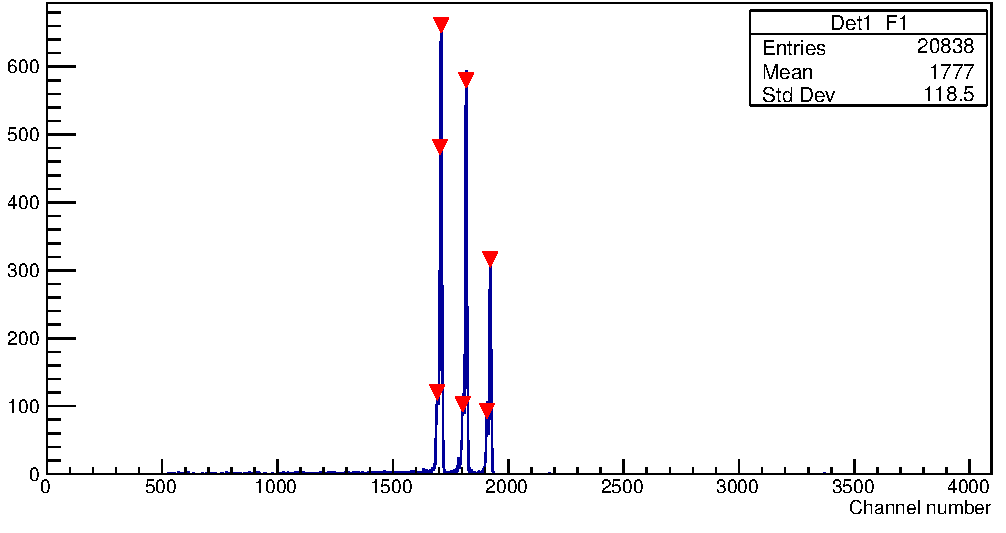
\includegraphics[width=\linewidth]{../figures/cali/det1f1-cropped.pdf}
	\caption{Calibration spectra from a front strip in Det1.}
	\label{fig:singleStripExample}
\end{figure}